\documentclass[aspectratio=169,10pt]{beamer}
\usepackage[T1]{fontenc}
\usepackage[utf8]{inputenc}
\usepackage[english]{babel}
\usepackage{lmodern}
\usepackage{booktabs}
\usepackage{array}
\usepackage{tikz}
\usetikzlibrary{arrows.meta,positioning,calc}

\definecolor{Ink}{HTML}{172B43}
\definecolor{Muted}{HTML}{526579}
\definecolor{Teal}{HTML}{087F8C}
\definecolor{Indigo}{HTML}{4956A3}
\definecolor{Amber}{HTML}{DD8D29}
\definecolor{Rust}{HTML}{AF4D35}
\definecolor{Pale}{HTML}{EFF4F7}
\definecolor{Line}{HTML}{DBE4EB}
\setbeamercolor{normal text}{fg=Ink,bg=white}
\setbeamercolor{structure}{fg=Teal}
\setbeamercolor{frametitle}{fg=Ink}
\setbeamercolor{alerted text}{fg=Rust}
\setbeamercolor{block title}{fg=Ink,bg=Pale}
\setbeamercolor{block body}{fg=Ink,bg=Pale}
\setbeamerfont{frametitle}{size=\Large,series=\bfseries}
\setbeamerfont{block title}{size=\normalsize,series=\bfseries}
\setbeamersize{text margin left=8mm,text margin right=8mm}
\setbeamertemplate{navigation symbols}{}
\setbeamertemplate{itemize item}{\color{Teal}\small\textbullet}
\setbeamertemplate{frametitle}{\vspace{3mm}\insertframetitle\par\vspace{1mm}\textcolor{Line}{\rule{\textwidth}{.5pt}}}
\setbeamertemplate{footline}{%
  \hspace{8mm}\textcolor{Muted}{\scriptsize SSBI · Task 3 · 20,000 PBMCs}\hfill
  \textcolor{Muted}{\scriptsize\insertframenumber}\hspace{8mm}\vspace{3mm}}
\setlength{\parskip}{2pt}
\newcommand{\takeaway}[1]{\vspace{2mm}\begin{beamercolorbox}[sep=1.7mm,wd=\linewidth]{block body}\small\textbf{#1}\end{beamercolorbox}}
\newcommand{\source}[1]{\vfill{\fontsize{6.5}{8}\selectfont\color{Muted}#1\par}}
\newcommand{\up}{\ensuremath{\uparrow}}
\newcommand{\down}{\ensuremath{\downarrow}}

\usepackage{amsmath,amssymb}
\definecolor{Best}{HTML}{157553}
\newcommand{\best}[1]{\textcolor{Best}{\textbf{#1}}}
\newcommand{\worst}[1]{\textcolor{Rust}{#1}}
%\newcommand{\PCOne}{12.60}
\newcommand{\PCTwo}{7.69}
\newcommand{\PCTogether}{20.29}
\newcommand{\PCSelected}{91.50}

\graphicspath{{figures/}}
\setbeamertemplate{footline}{\hspace{8mm}\textcolor{Muted}{\scriptsize SSBI · Dimensionality Reduction}\hfill\textcolor{Muted}{\scriptsize\insertframenumber}\hspace{8mm}\vspace{3mm}}
\hypersetup{pdftitle={Task 2: Dimensionality reduction},pdfauthor={SSBI group project}}
% --- add to the preamble, once, before \begin{document} ---
\newcommand{\seminar}[1]{\def\myseminar{#1}}
\newcommand{\supervisor}[1]{\def\mysupervisor{#1}}

\title{Benchmark of comparative single-cell analysis approaches}
%\subtitle{YOUR SUBTITLE HERE}
\author{Gregor Habitzreither \and Sebastian Fay  \and Marie Schygulla}
\date{11. September 2026}
\seminar{Structure Teamproject 2026}
\supervisor{Prof. Dr. Manfred Claassen}

\begin{document}

\begin{frame}[plain]
  \begin{center}
    \vspace{6mm}
    {\usebeamercolor[fg]{title}\LARGE\bfseries\inserttitle}\par
    \vspace{2mm}
    \ifx\insertsubtitle\@empty\else
      {\usebeamercolor[fg]{title}\large\insertsubtitle}\par
      \vspace{8mm}
    \fi
    {\large\insertauthor}\par
    \vspace{8mm}
    {\normalsize\myseminar}\par
    {\normalsize Supervised by \mysupervisor ~and Pouria Laghaee}\par
    \vspace{6mm}
    {\normalsize\insertdate}
  \end{center}
\end{frame}

\begin{frame}{Benchmark of comparative single-cell analysis approaches}
  \begin{columns}[T,onlytextwidth]
  \begin{column}{.45\textwidth}
    \textcolor{Teal}{\large The Data}\par\medskip
    from Horowitz et al. (2013)
    \par\medskip
    \begin{tabular}{lr}\toprule
      Provided donors & 20\\
      CMV+/CMV- & 9/11\\
      Analysis markers & 37\\
      Available gated NK cells & 261,593\\
      Balanced analysis sample & 40,000\\\bottomrule
    \end{tabular}
  \end{column}
  \begin{column}{.42\textwidth}
    \textcolor{Teal}{\large The context}\par\medskip
    \textbf{Mass cytometry (CyTOF)}: simultaneous protein-marker measurements on individual cells.
    \textbf{Natural Killer (NK) cells}: immune cells with a high cell diversity
    \par\medskip
    From some donors a subpopulation of NK cells shows a characteristic expression of proteins typical after a CMV infection, which was given in the data
    \par\medskip
  \end{column}
  \end{columns}
  \takeaway{CMV labels describe donors; they do not identify infected individual cells.}
  \source{Horowitz et al., Sci. Transl. Med. 2013; Arvaniti \& Claassen, Nat. Commun. 2017. Provided 20-donor subset}
\end{frame}

\begin{frame}{Does the balanced subsample preserve the selected phenotype?}
  \begin{columns}[c,onlytextwidth]
  \begin{column}{.49\textwidth}
    \centering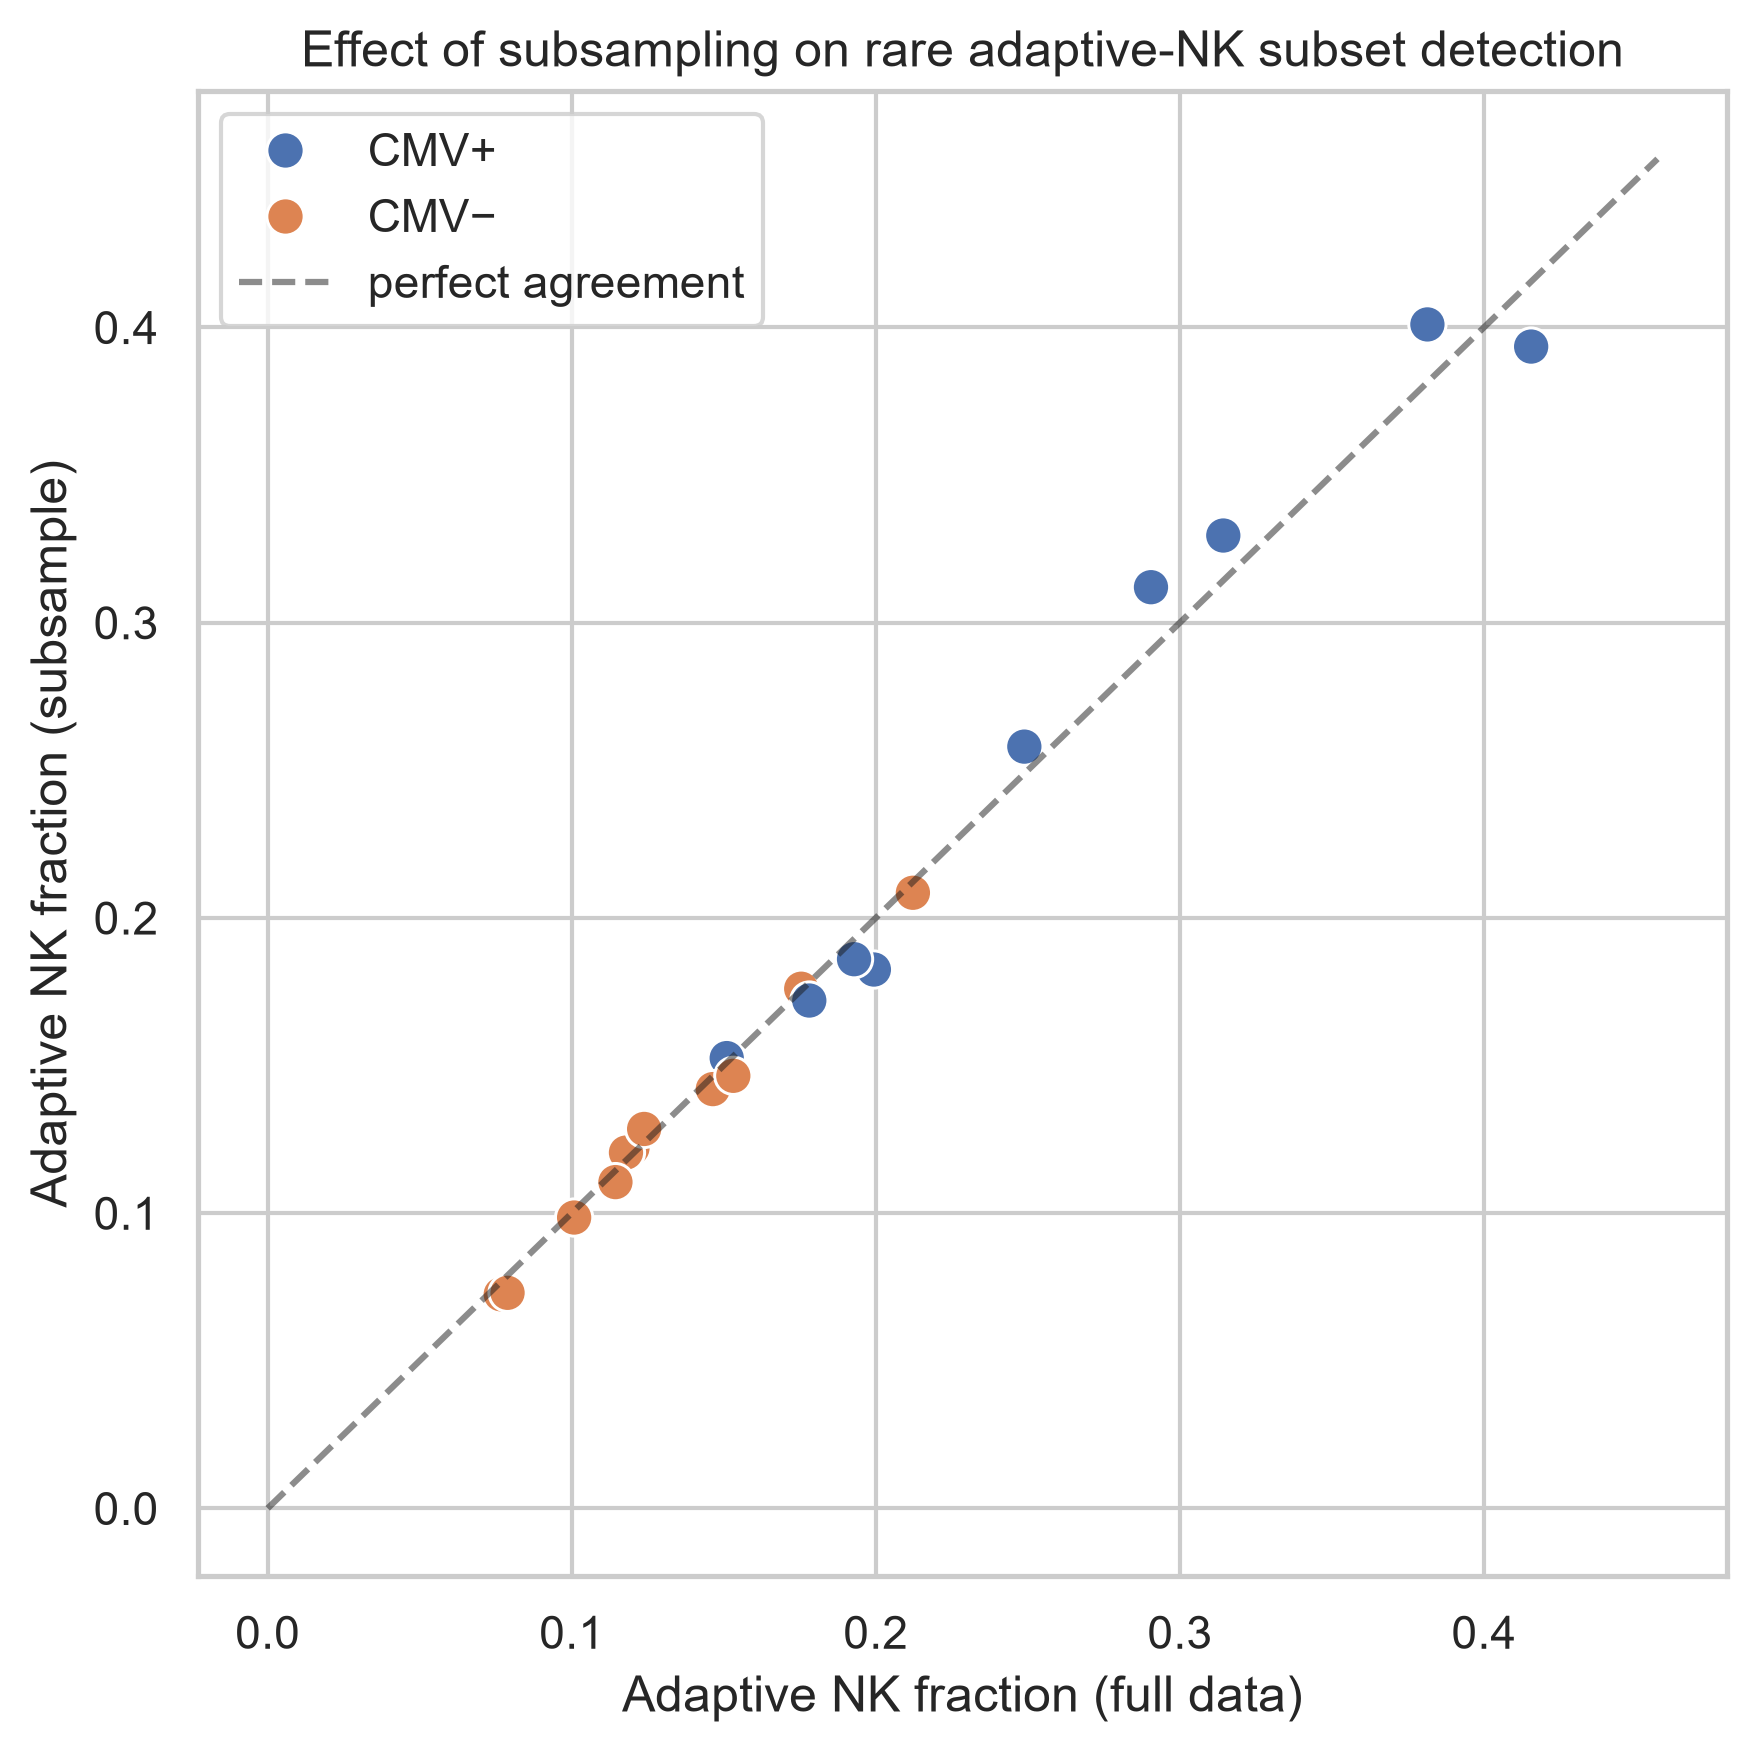
\includegraphics[height=54mm]{subsample.png}
  \end{column}
  \begin{column}{.47\textwidth}
    Compare randomly choosen \textbf{2,000 cells per donor} with all available gated NK cells from that donor.\par\medskip
    NKG2C$^+$/CD57$^+$ is a marker phenotype associated with \textbf{memory-like (``adaptive'') NK cells} after CMV exposure.
  \end{column}
  \end{columns}
  \source{Positivity: two-component GMM crossover per marker on all 261,593 cells. This check concerns one approximate phenotype, not every rare population.}
\end{frame}

\begin{frame}{PCA}
  \begin{columns}[c,onlytextwidth]
  \begin{column}{.45\textwidth}
    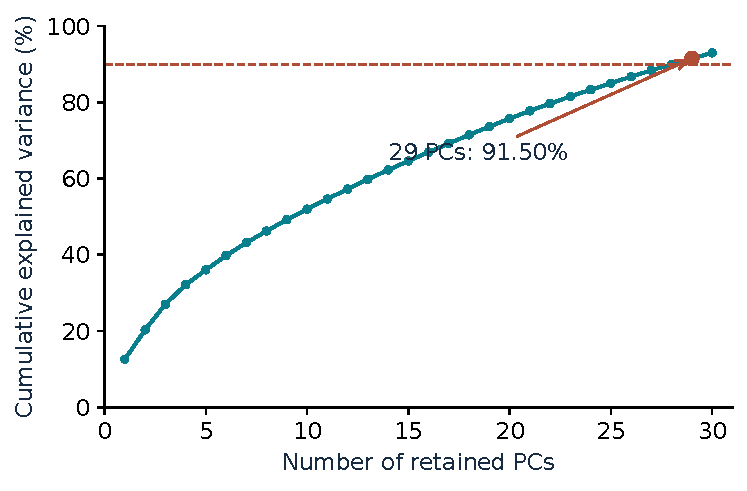
\includegraphics[width=\linewidth]{pca_spectrum.pdf}
  \end{column}
  \begin{column}{.53\textwidth}
    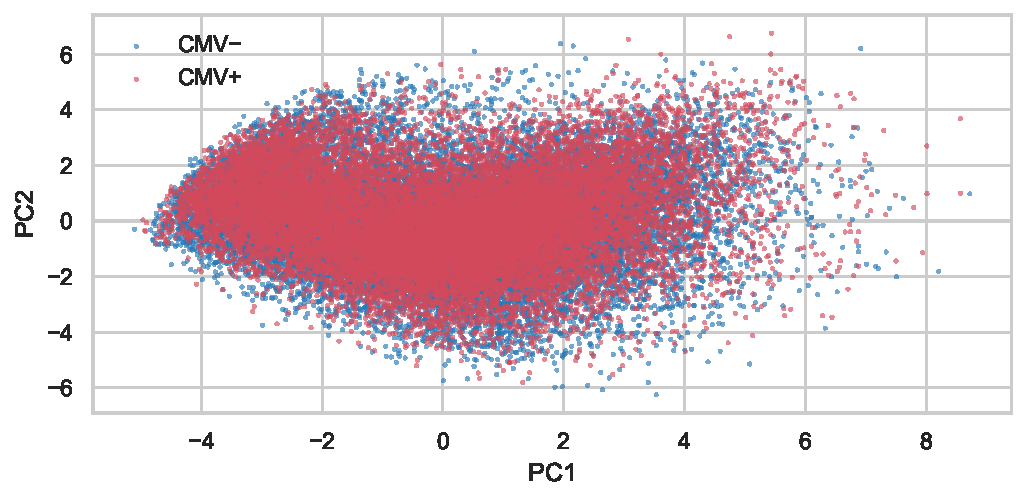
\includegraphics[width=\linewidth]{pca_donor.pdf}
  \end{column}
  \end{columns}
  \medskip
  \textbf{Retention choice:} 29 PCs reach the 90\% threshold and become the input to t-SNE/UMAP.\par
  \takeaway{29 PCs retain 91.50\%, the plotted two retain only 20.29\%}
  \source{40,000 cells, arcsinh + z-scoring. Spectrum verified from the same 37-marker covariance matrix}
\end{frame}

\begin{frame}{t-SNE: changing perplexity changes the neighbourhood scale}
  \centering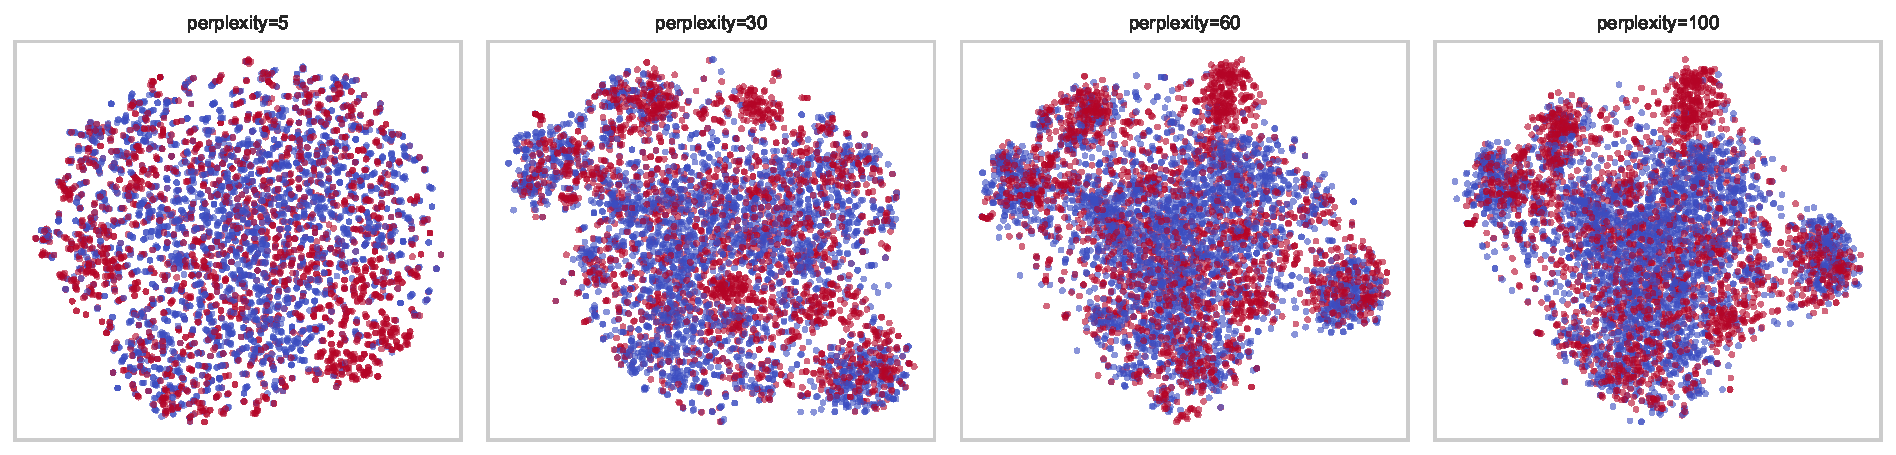
\includegraphics[height=36mm]{tsne_selected.pdf}\par\smallskip
  \begin{columns}[T,onlytextwidth]
  \begin{column}{.40\textwidth}\small
    \textbf{Input}:
    5,000 cells and 29 PCs reduce sweep time and memory. 
    \par\smallskip
    The top-scoring of 5, 15, 30, 40, 50, 60, 70 and 100. \textbf{Selected: 60}
  \end{column}
  \begin{column}{.50\textwidth}\small
    \centering
    \begin{tabular}{rr}\toprule
      Perplexity & Trustworthiness\\\midrule
      50 & 0.92597\\
      60 & 0.92605\\
      100 & 0.92580\\\bottomrule
    \end{tabular}\\[2pt]
    \par\smallskip
    \raggedright $T$: penalises false low-dimensional neighbours by their high-dimensional ranks.
  \end{column}
  \end{columns}
  \source{Selected panels; colours indicate donor CMV status.}
\end{frame}

\begin{frame}{UMAP}
  \begin{columns}[c,onlytextwidth]
  \begin{column}{.40\textwidth}
    \centering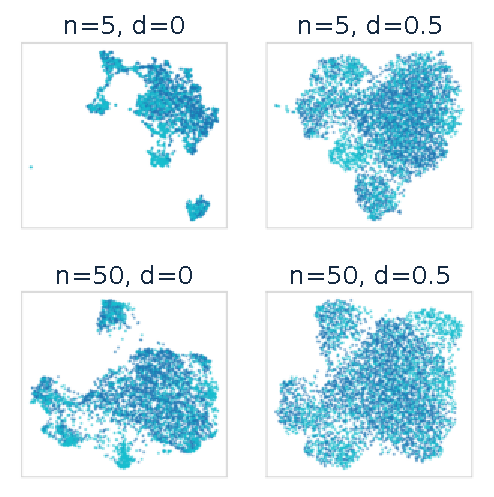
\includegraphics[height=51mm]{umap_selected.pdf}
  \end{column}
  \begin{column}{.60\textwidth}
    \begin{center}
      \small\begin{tabular}{rrr}\toprule
$n_{\rm neighbors}$ & min\_dist & $T(15)$\\\midrule
5 & 0.0 & 0.890139\\
5 & 0.1 & 0.879145\\
30 & 0.0 & 0.877151\\
\bottomrule\end{tabular}
\par\medskip
    \end{center}
    \normalsize Selected: \textbf{5 neighbours, min\_dist = 0.0}. %Compact islands do not prove distinct cell types.
  \end{column}
  \end{columns}
  \source{Four corner settings from the 16-panel saved grid, colours indicate CMV status. Top three rows ranked by saved Trustworthiness on the same 5,000 cells and 29 PCs.}
\end{frame}

\begin{frame}{Local preservation and global distances favour different maps}
  \begin{columns}[c,onlytextwidth]
  \begin{column}{.60\textwidth}
  \centering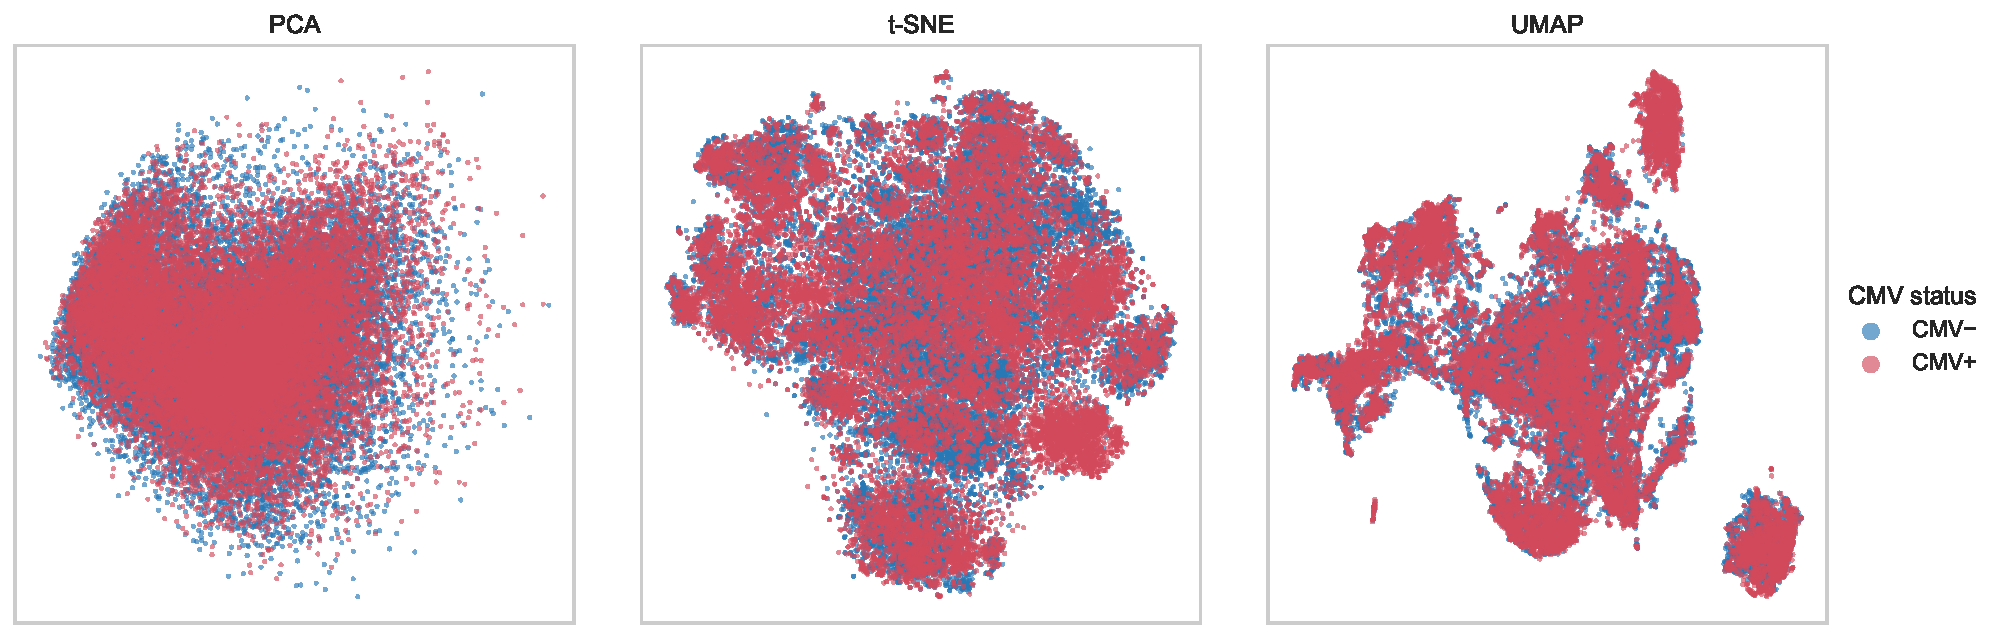
\includegraphics[width=.90\textwidth,height=26mm,keepaspectratio]{embeddings_cmv.pdf}\par
  \smallskip\small\begin{tabular}{lrrrr}\toprule
Embedding & $T(15)\uparrow$ & $R(15)\uparrow$ & $r_d\uparrow$ & $S_{\rm CMV}\uparrow$\\\midrule
PCA & \worst{0.7258} & \worst{0.0072} & \best{0.6204} & \worst{0.0016}\\
t-SNE & \best{0.9612} & \best{0.2232} & 0.4868 & 0.0104\\
UMAP & 0.9009 & 0.1126 & \worst{0.3954} & \best{0.0178}\\
\bottomrule\end{tabular}
\par\smallskip
  \end{column}
  \begin{column}{.38\textwidth}
    \begin{minipage}{\linewidth}\scriptsize
    \textcolor{Teal}{\textbf{Local structure}}\par
    $T$: \textbf{Trustworthiness} -- false neighbours, ranked.\par \smallskip
    $R$: \textbf{kNN preservation} -- exact overlap; small values are normal at $n=40{,}000$ (chance level $\approx 0.0004$).\par \smallskip
    {\itshape t-SNE wins both: it directly optimises neighbour probabilities.}\par
    \vspace{5pt}\hrule\vspace{5pt}
    \textcolor{Teal}{\textbf{Global / label structure}}\par
    $r_d$: \textbf{Pearson correlation} of all pairwise distances.\par
    {\itshape PCA wins: a linear projection built to preserve overall variance/distance.}\par \smallskip
    $S_{\rm CMV}$: \textbf{Silhouette score} - separation by donor CMV label -- near zero for all three maps, as expected: only a minority subset of each CMV+ donor's cells is actually altered.
    \end{minipage}
  \end{column}
  \end{columns}
  \takeaway{t-SNE leads locally; PCA leads in distance correlation.}
  \source{40,000 cells; 29 PCs; k=15. Distance correlation: fixed 2,000-cell sample.}
\end{frame}

\begin{frame}{Which maps are most similar?}
  \begin{columns}[c,onlytextwidth]
  \begin{column}{.51\textwidth}
    \begin{center}
      \small\begin{tabular}{lrr}\toprule
Pair & $R(15)\uparrow$ & $M^2\downarrow$\\\midrule
PCA vs t-SNE & 0.00585 & \best{0.45189}\\
PCA vs UMAP & \worst{0.00410} & \worst{0.73390}\\
t-SNE vs UMAP & \best{0.12532} & 0.72369\\
\bottomrule\end{tabular}
\par\smallskip
      {\scriptsize $R$ values look small in absolute terms, but sit far above the $\sim0.0004$ level expected by chance at $n=40{,}000$, $k=15$.}
    \end{center}
    \par\medskip
  
  \end{column}
  \begin{column}{.44\textwidth}
      \textcolor{Teal}{\textbf{$M^2$ -- Procrustes disparity}}\par\smallskip
    \small Align two maps by translation, rotation/reflection and scaling; measure the remaining mismatch. Lower = closer overall shape after alignment.\par
    \vspace{5pt}\hrule\vspace{5pt}
    \textbf{Local neighbours ($R$):} t-SNE and UMAP are the most similar pair.\par\medskip
    \textbf{Aligned global shape ($M^2$):} PCA and t-SNE are the most similar pair. \par \medskip
  \end{column}
  \end{columns}
  \takeaway{$R$ and $M^2$ disagree because they ask different questions: exact shared neighbours vs. overall shape after optimal alignment}
  \source{All three pairs evaluated on the same 40,000 cells in the same order. R(15) corrected from saved coordinates; SciPy Procrustes values independently reproduced. Neither metric identifies biologically correct cell types.}
\end{frame}

\appendix

\begin{frame}{Backup: Data Transformation and z-scoring}
  \begin{columns}[c,onlytextwidth]
  \begin{column}{.58\textwidth}
    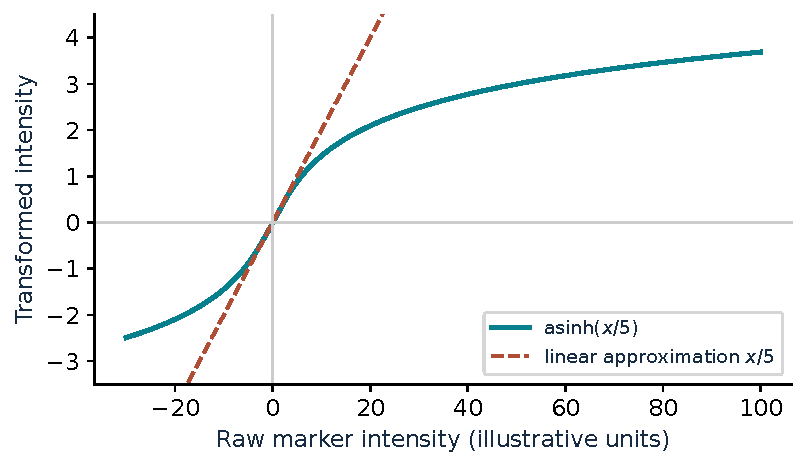
\includegraphics[width=\linewidth]{figures/arcsinh.pdf}
  \end{column}
  \begin{column}{.38\textwidth}
    \textcolor{Teal}{\large The arcsinh transformation}
    \[a_{ij}=\operatorname{asinh}(x_{ij}/5)\]
    Approximately linear near zero; compresses large magnitudes and accepts negative background values.\par\medskip
    \textcolor{Teal}{\large Marker-wise z-scoring}
    \[z_{ij}=\frac{a_{ij}-\bar a_j}{s_j}\]
    Prevents large marker scales from dominating distances. All 37 markers pass the variance (0.05) filter.
  \end{column}
  \end{columns}
  \source{cofactor 5; pooled scaling across the balanced exploratory sample. Curve is a mathematical illustration.}
\end{frame}

\begin{frame}{Backup: how t-SNE turns neighbours into a map}
  \begin{columns}[T,onlytextwidth]
  \begin{column}{.46\textwidth}
    \setlength{\abovedisplayskip}{2pt}\setlength{\belowdisplayskip}{2pt}
    High-D affinity (probability that $j$ is a neighbour of $i$):
    \[p_{ij}\propto\exp(-\lVert x_i-x_j\rVert^2/2\sigma_i^2)\]
    Low-D affinity (heavy-tailed, avoids "crowding"):
    \[q_{ij}\propto(1+\lVert y_i-y_j\rVert^2)^{-1}\]
    Optimisation moves points in 2D until $q_{ij}$ matches $p_{ij}$ as closely as possible (minimises $\mathrm{KL}(P\Vert Q)$).\par\smallskip
    $\sigma_i$ is tuned per point so its affinities imply the chosen perplexity.
  \end{column}
  \begin{column}{.50\textwidth}
    \footnotesize
    \begin{tabular}{lp{.74\textwidth}}\toprule
      \textbf{perplexity} & swept (5--100); effective neighbourhood size -- see main slide.\\
      \textbf{init = pca} & starts from the PCA layout instead of random noise: more reproducible, avoids poor local optima.\\
      \textbf{learning rate = auto} & optimiser step size; scikit-learn scales it with sample size.\\
      \textbf{early exagg. = 12} & temporarily inflates high-D affinities early on, so initial clusters separate before fine positioning.\\
      \textbf{angle = 0.5} & Barnes--Hut speed/accuracy trade-off; a numerical setting, not a property of the data.\\
      \textbf{max\_iter = 750} & fixed iteration budget -- not itself a convergence check (see caveat below).\\\bottomrule
    \end{tabular}
  \end{column}
  \end{columns}
  \source{van der Maaten \& Hinton (2008); scikit-learn TSNE documentation. A fixed iteration count alone does not confirm convergence. Defaults refer to the documented scikit-learn 1.9 environment.}
\end{frame}

\begin{frame}{Backup: kNN preservation (R)}
  Let $N_i^X(k)$, $N_i^Y(k)$ be the $k$ nearest neighbours of cell $i$ in the high-D
  reference $X$ and the embedding $Y$ (excluding itself).
  \[
    R(k)=\frac{1}{n}\sum_{i=1}^n\frac{|N_i^X(k)\cap N_i^Y(k)|}{k}
  \]
  \small Symmetric; counts exact shared identities, not just "close enough."\par\medskip
  \textcolor{Teal}{\textbf{What $k$ controls.}} How many neighbours count as "local." Small $k$
  is a strict test of fine-grained ordering; large $k$ is a looser test that tolerates more
  reshuffling and starts to resemble cluster-membership agreement rather than precise
  neighbour identity.\par\smallskip
  \textcolor{Teal}{\textbf{Why $k=15$ here.}} Fixed throughout to match the neighbourhood scale
  explored in the UMAP sweep (\texttt{n\_neighbors} 5--50) and sits within the commonly used
  10--30 range for trustworthiness-style scores at this dataset size.\par\medskip
  \textbf{Example:} ten shared neighbours out of fifteen contribute $10/15$.\par\smallskip
  \source{Venna \& Kaski (2001); scikit-learn NearestNeighbors documentation. Full-sample scores average over cells; equal cells per donor give equal donor weight.}
\end{frame}

\begin{frame}{Backup: Trustworthiness (T)}
  Using the same $k=15$ and the same neighbour sets $N_i^X(k)$, $N_i^Y(k)$ as $R$:
  \[
    T(k)=1-\frac{2}{nk(2n-3k-1)}\sum_i\sum_{j\in N_i^Y(k)\setminus N_i^X(k)}(r_X(i,j)-k)
  \]
  \small Penalises \emph{false} low-D neighbours (points that look close in the embedding but
  weren't close in the reference) according to how far out of the true top-$k$ they actually
  ranked. Unlike $R$, direction matters here: $T$ only punishes false positives, not missed
  true neighbours.\par\medskip
  \textbf{Example:} a false neighbour originally ranked 16th (just outside the true top-15)
  contributes only $(16-15)=1$ to the penalty; one ranked 500th contributes 485 -- a much larger
  embedding error is penalised much more heavily.
  \source{Venna \& Kaski (2001); scikit-learn trustworthiness documentation. Here $k=15$, matching $R$.}
\end{frame}

\begin{frame}{Backup: how UMAP constructs and embeds a weighted graph}
  \small
  \[w_{j|i}=\exp\!\left[-\frac{\max(0,d(x_i,x_j)-\rho_i)}{\sigma_i}\right],\qquad
    w_{ij}=w_{j|i}+w_{i|j}-w_{j|i}w_{i|j}.\]
  Offset $\rho_i$ and scale $\sigma_i$ adapt to local density; directed neighbourhoods are combined into symmetric weights.\par
  \[v_{ij}=(1+a\lVert y_i-y_j\rVert^{2b})^{-1},\qquad
    L\sim-\sum_{i<j}\{w_{ij}\log v_{ij}+(1-w_{ij})\log(1-v_{ij})\}.\]
  Sampled updates balance attraction and repulsion. The parameters $a,b$ depend on min\_dist and spread.\par\smallskip
  \begin{tabular}{lp{.67\textwidth}}\toprule
    Swept & n\_neighbors: 5, 15, 30, 50; min\_dist: 0, 0.1, 0.3, 0.5.\\
    Fixed/default & 2 dimensions, seed 42, Euclidean metric, spectral initialisation, spread 1.\\\bottomrule
  \end{tabular}\par\smallskip
  Larger neighbourhoods change the scale of the graph; larger min\_dist discourages tight packing. Neither guarantees accurate global distances.
  \source{McInnes, Healy \& Melville (2018/2020); official UMAP parameter and algorithm documentation. Equations describe the conceptual objective, not every optimisation approximation.}
\end{frame}

\begin{frame}{Backup: how UMAP constructs and embeds a weighted graph}
  \small
  \textcolor{Teal}{\textbf{Step 1 -- build the high-D graph.}}
  \[w_{j|i}=\exp\!\left[-\frac{\max(0,d(x_i,x_j)-\rho_i)}{\sigma_i}\right],\qquad
    w_{ij}=w_{j|i}+w_{i|j}-w_{j|i}w_{i|j}.\]
  Offset $\rho_i$ and scale $\sigma_i$ \textbf{adapt to local density}; directed neighbourhoods
  are combined into symmetric edge weights.\par\medskip
  \textcolor{Teal}{\textbf{Step 2 -- fit a low-D layout to match it.}}
  \[v_{ij}=(1+a\lVert y_i-y_j\rVert^{2b})^{-1},\qquad
    L\sim-\sum_{i<j}\{w_{ij}\log v_{ij}+(1-w_{ij})\log(1-v_{ij})\}.\]
  Sampled updates balance \textbf{attraction} (true neighbours pulled together) and
  \textbf{repulsion} (non-neighbours pushed apart). $a,b$ are fit automatically from
  \texttt{min\_dist}/\texttt{spread}, not set directly.\par\smallskip
  \begin{tabular}{lp{.67\textwidth}}\toprule
    \textcolor{Teal}{Swept} & \textbf{n\_neighbors}: 5, 15, 30, 50; \textbf{min\_dist}: 0, 0.1, 0.3, 0.5.\\
    \textcolor{Teal}{Fixed/default} & 2 dimensions, seed 42, Euclidean metric, spectral initialisation, spread 1.\\\bottomrule
  \end{tabular}\par\smallskip
  Larger neighbourhoods change the \textbf{scale} of the graph; larger \texttt{min\_dist}
  discourages tight packing. Neither guarantees accurate global distances.
  \source{McInnes, Healy \& Melville (2018/2020); official UMAP parameter and algorithm documentation. Equations describe the conceptual objective, not every optimisation approximation.}
\end{frame}

\begin{frame}{Backup: UMAP sweep, 5 and 15 neighbours}
  \centering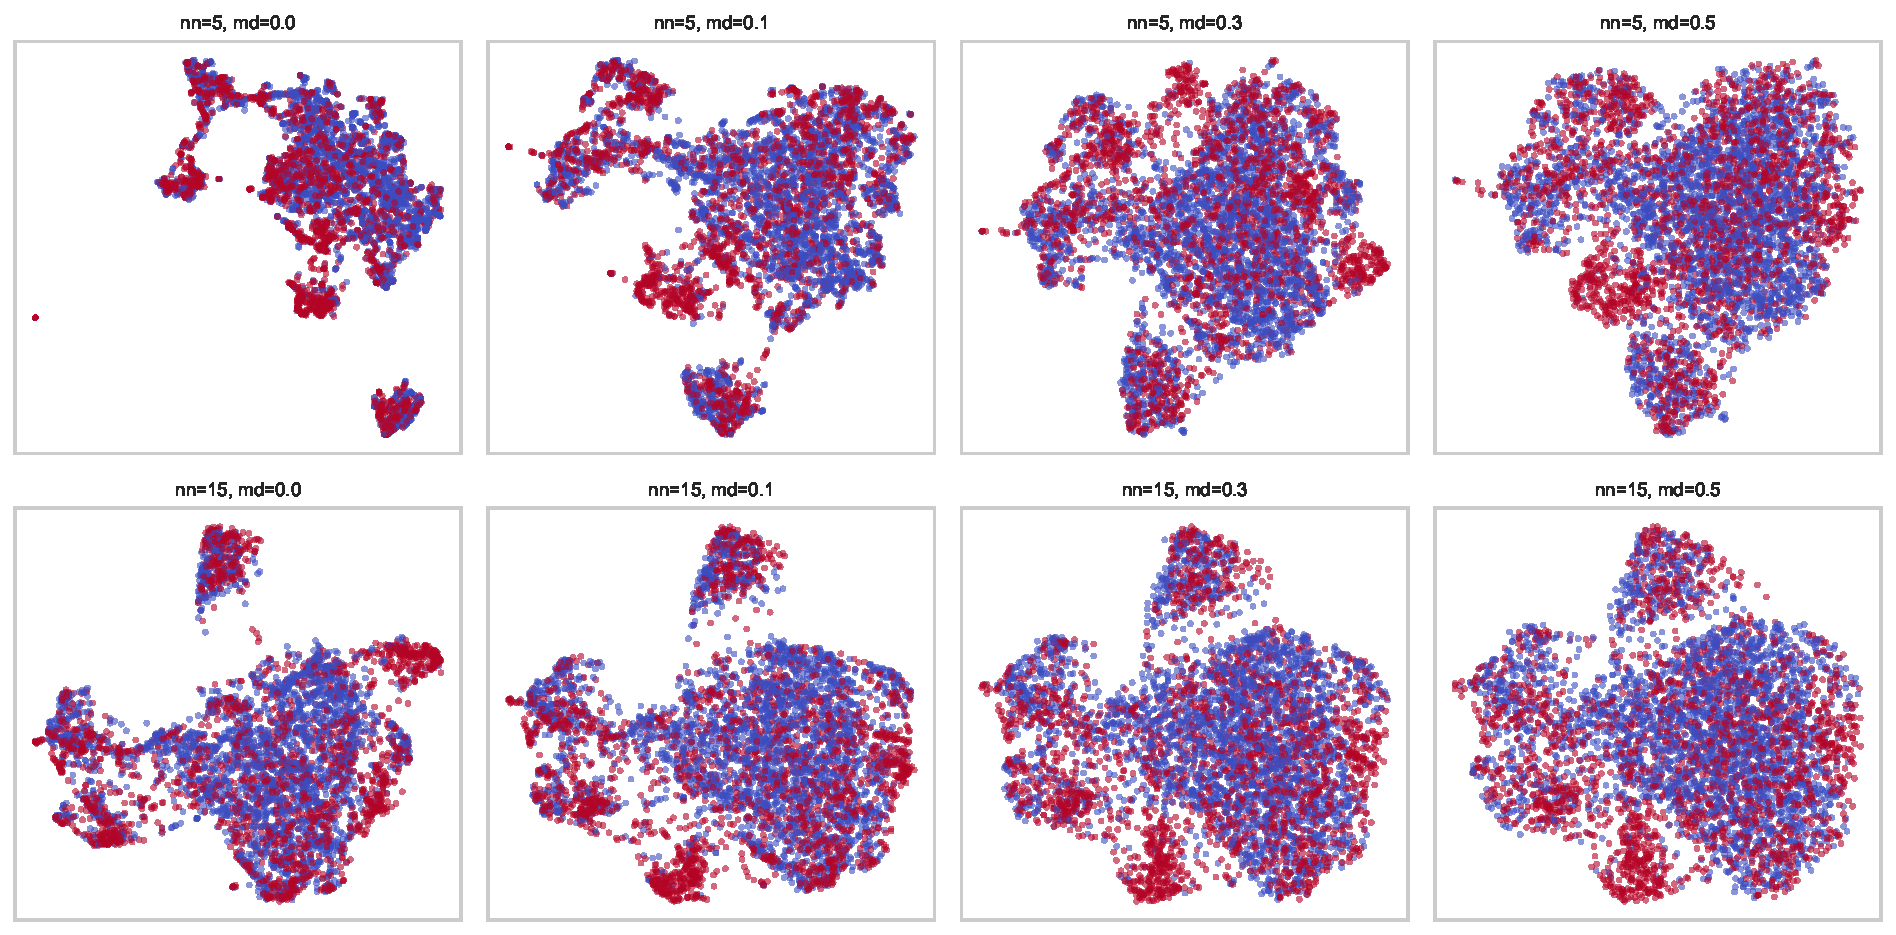
\includegraphics[width=.96\textwidth,height=60mm,keepaspectratio]{umap_grid_1.pdf}
\source{Rows 1--2 of the original 16-panel grid. Same 5,000 cells, 29 PCs, seed 42;  Visual changes are parameter effects within one run, not a stability study across seeds.}
\end{frame}

\begin{frame}{Backup: UMAP sweep, 30 and 50 neighbours}
  \centering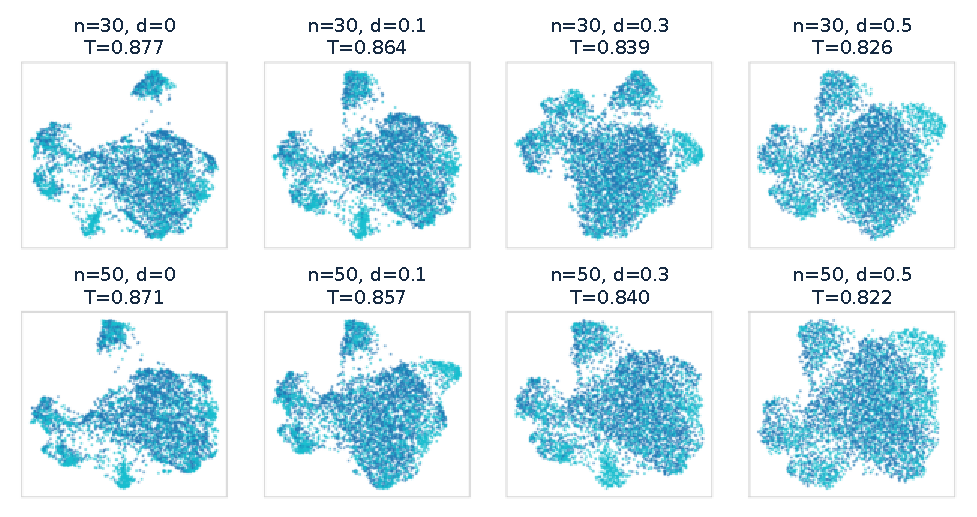
\includegraphics[width=.96\textwidth,height=60mm,keepaspectratio]{umap_grid_2.pdf}
\source{Rows 3--4 of the original 16-panel grid. Same 5,000 cells, 29 PCs, seed 42; Visual changes are parameter effects within one run, not a stability study across seeds.}
\end{frame}

\begin{frame}{Backup: the same markers on the t-SNE map}
  \centering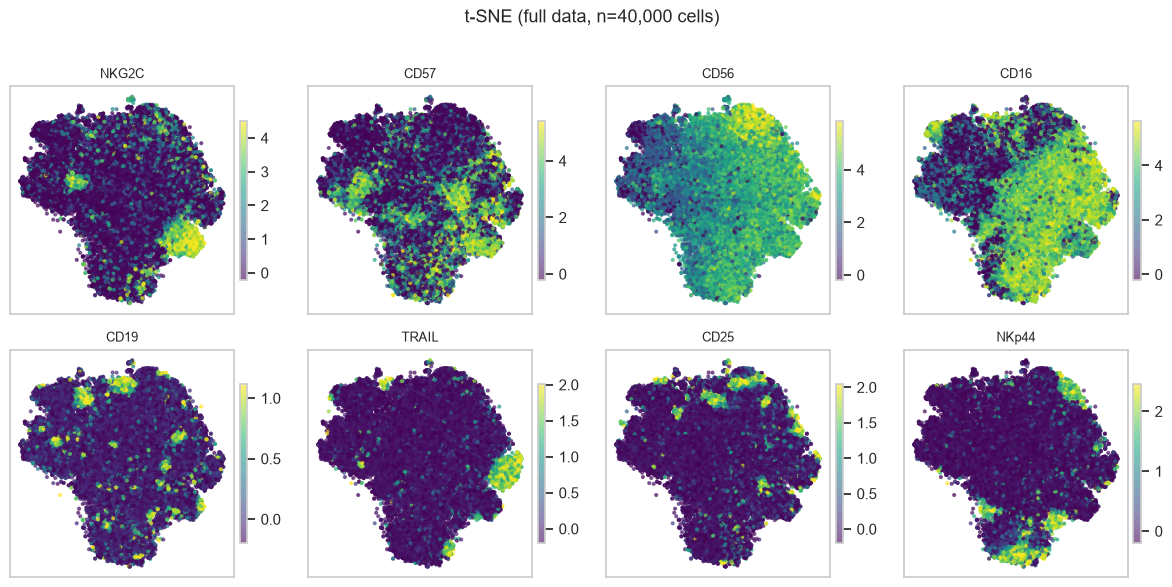
\includegraphics[width=.98\textwidth,height=56mm,keepaspectratio]{tsne_markers.png}
\source{40,000 balanced cells. Arcsinh-transformed marker values; colour limits use the 1st/99th percentiles separately per marker. A bright region does not establish an infected-cell population.}
\end{frame}

\begin{frame}{Backup: marker expression on the UMAP map}
  \centering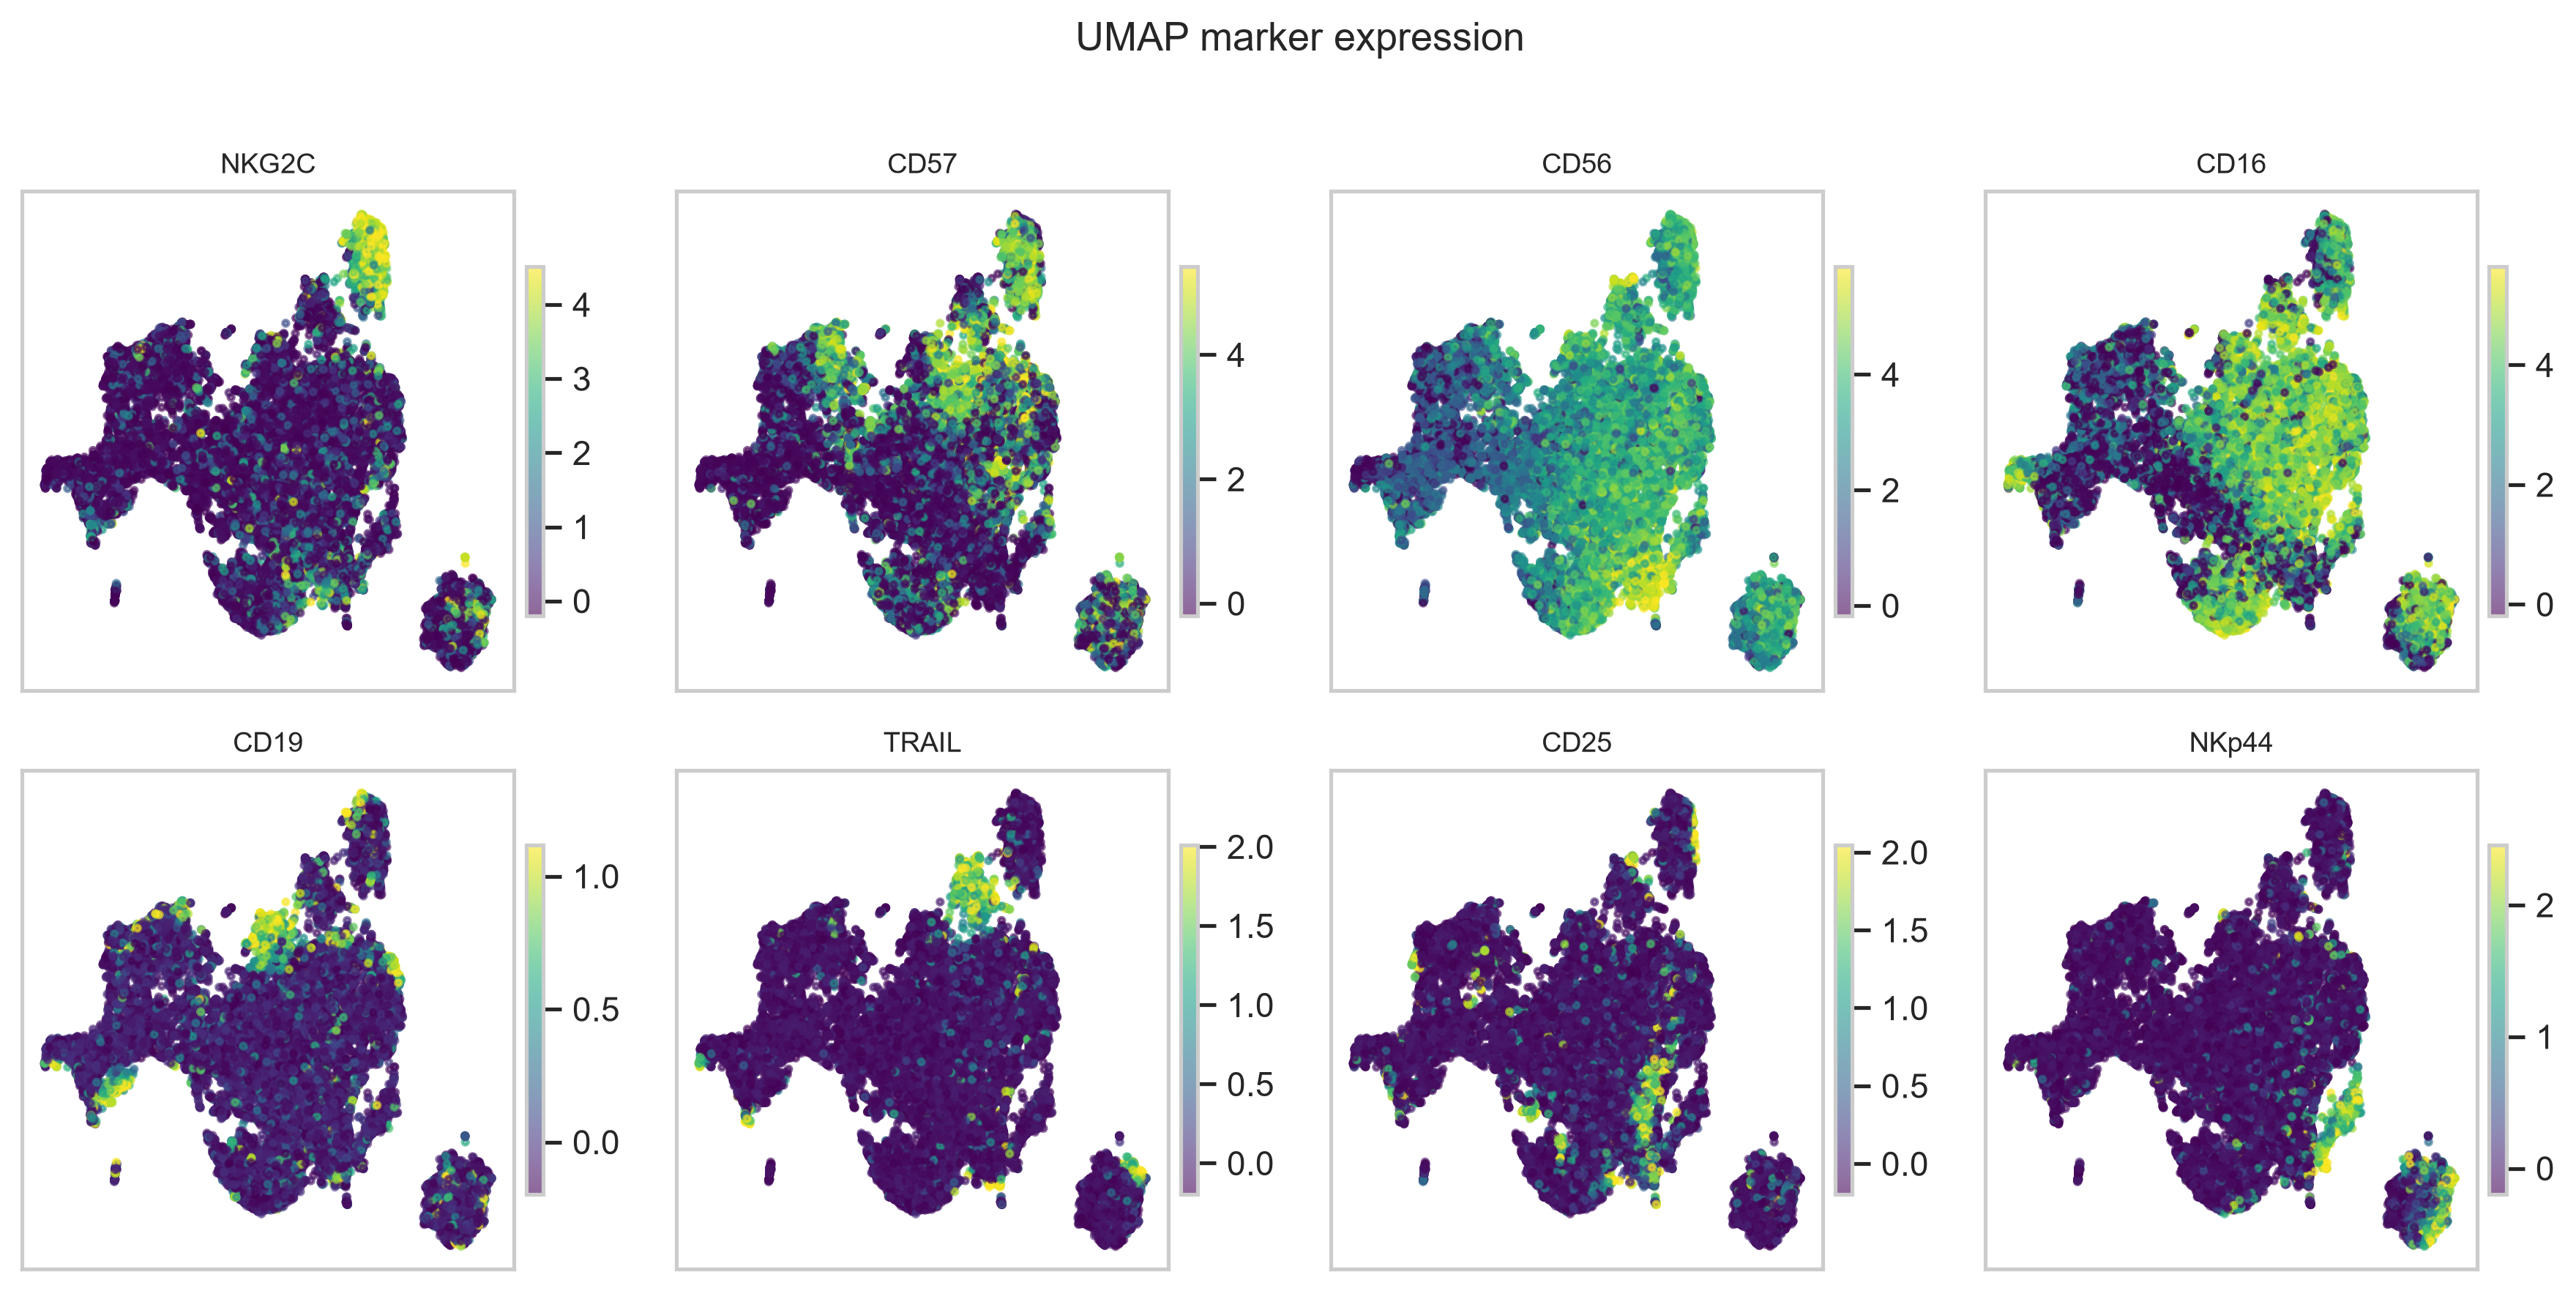
\includegraphics[width=.98\textwidth,height=56mm,keepaspectratio]{umap_markers.png}
\source{40,000 balanced cells. Arcsinh-transformed marker values; colour limits use the 1st/99th percentiles separately per marker. A bright region does not establish an infected-cell population.}
\end{frame}

\begin{frame}{Backup: Shepard diagram to compare distances}
  \centering
  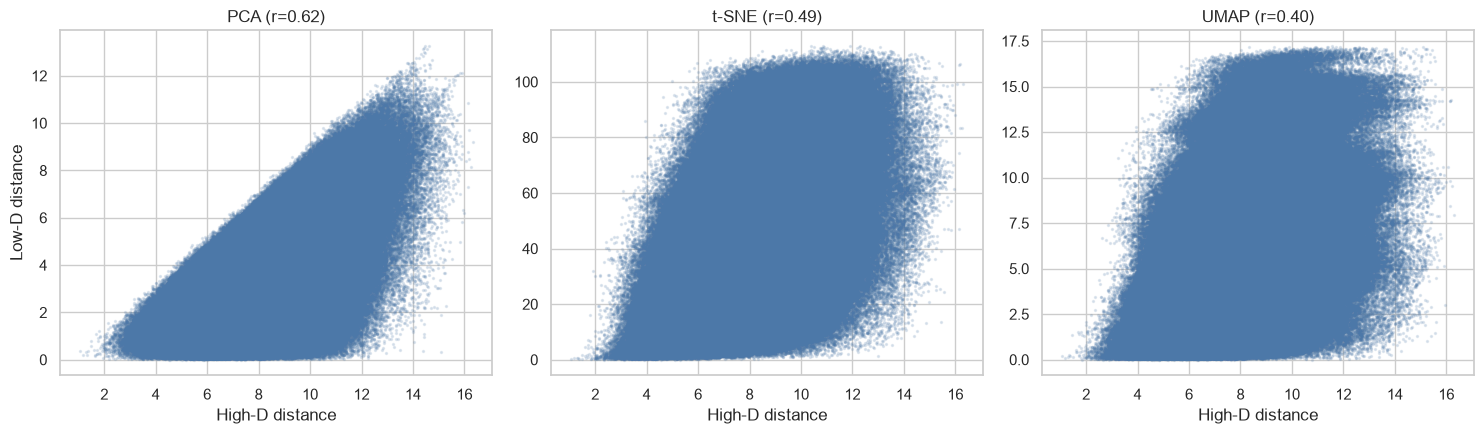
\includegraphics[
    width=0.88\textwidth,
    height=48mm,
    keepaspectratio
  ]{shepard.png}
  \vspace{2mm}
  \begin{columns}[T,onlytextwidth]
    \begin{column}{0.48\textwidth}
      \scriptsize
      Each point represents one sampled cell pair. The \textbf{horizontal axis} is the distance in the 29-dimensional PCA reference space. \par \smallskip
      The \textbf{vertical axis} is the distance in the two-dimensional embedding.
      Pearson correlation measures agreement in relative distances.
    \end{column}
    \begin{column}{0.48\textwidth}
      \scriptsize
      UMAP's loss doesn't optimize for preserving absolute distances at all, and \texttt{min\_dist}=0 actively encourages tight packing, so many far-apart high-D pairs get compressed into a similar low-D distance ceiling $\rightarrow$ lowest $r_d$ of the three
    \end{column}
  \end{columns}
  \source{Fixed 2,000-cell sample; 29-PC reference space; Pearson correlation of pairwise distances.}
\end{frame}

\begin{frame}{Backup: Procrustes aligns the maps before measuring mismatch}
  Centre and normalise each coordinate matrix to unit Frobenius norm:
  \[ A_c=\frac{A-\bar A}{\lVert A-\bar A\rVert_F},\qquad B_c=\frac{B-\bar B}{\lVert B-\bar B\rVert_F}.\]
  \[M^2=\min_{s,Q:\,Q^\top Q=I}\lVert A_c-sB_cQ\rVert_F^2.\]
  \smallskip
  \begin{itemize}
    \item Rows must correspond to exactly the same cells in the same order.
    \item Rotation/reflection, translation and uniform scaling do not count as biological differences.
    \item Lower disparity means a closer global fit after alignment; it does \textbf{not} establish local fidelity (whether each point's \emph{immediate} neighbours are correctly placed -- that's what $T$/$R$ measure instead) or class separation.
    \item Nonlinear deformations can change neighbour identities and global shape differently.
  \end{itemize}
  \source{SciPy scipy.spatial.procrustes. With its normalisation and optimal scaling, the scalar disparity is symmetric even though the returned transformed matrices have different normalisation conventions.}
\end{frame}

\begin{frame}{Sources}
  \small
  \textbf{Data and biology}\par
  Horowitz et al. (2013). \emph{Genetic and environmental determinants of human NK cell diversity revealed by mass cytometry.} Sci. Transl. Med. 5:208ra145.\par
  Arvaniti \& Claassen (2017). \emph{Sensitive detection of rare disease-associated cell subsets via representation learning.} Nat. Commun. 8:14825.\par\medskip
  \textbf{Methods}\par
  van der Maaten \& Hinton (2008), JMLR 9:2579--2605 (t-SNE).\par
  McInnes, Healy \& Melville (2018/2020), arXiv:1802.03426 (UMAP).\par
  Venna \& Kaski (2001), ICANN, pp. 485--491 (Trustworthiness).\par
  Official scikit-learn and SciPy documentation; linked references in the detailed report.\par\medskip
\end{frame}
\end{document}
